\documentclass[aspectratio=169]{beamer}

\usetheme{Madrid}
\usecolortheme{default}

\usepackage{booktabs}
\usepackage{tikz}
\usepackage{hyperref}

% Time formatting
\newcount\myhours
\newcount\myminutes
\myhours=\time \divide\myhours by 60
\myminutes=\time \multiply\myhours by 60 \advance\myminutes by -\myhours
\divide\myhours by 60
\def\mytime{\ifnum\myhours<10 0\fi\the\myhours:\ifnum\myminutes<10 0\fi\the\myminutes}

\title{SpeakUp}
\subtitle{A Systems-Engineering Demonstration}
\author{Bruce Dombrowski}
\date{December 22, 2025}

% Footer with repo link
\setbeamertemplate{footline}{
  \leavevmode%
  \hbox{%
  \begin{beamercolorbox}[wd=.333333\paperwidth,ht=2.25ex,dp=1ex,center]{author in head/foot}%
    \usebeamerfont{author in head/foot}\insertshortauthor
  \end{beamercolorbox}%
  \begin{beamercolorbox}[wd=.333333\paperwidth,ht=2.25ex,dp=1ex,center]{title in head/foot}%
    \usebeamerfont{title in head/foot}\insertshorttitle
  \end{beamercolorbox}%
  \begin{beamercolorbox}[wd=.333333\paperwidth,ht=2.25ex,dp=1ex,right]{date in head/foot}%
    \usebeamerfont{date in head/foot}\insertframenumber{} / \inserttotalframenumber\hspace*{2ex}
  \end{beamercolorbox}}%
  \vskip0pt%
}

\begin{document}

\begin{frame}
\titlepage
\vspace{-1em}
\begin{center}
\small
Repository: \url{https://github.com/brucedombrowski/SpeakUp}\\
\vspace{0.3em}
\scriptsize Generated: \today\ \mytime
\end{center}
\end{frame}

\begin{frame}{About This Document}
\textbf{Purpose:} This briefing is designed for asynchronous review by managers and customers. It can be read independently without a presenter.

\vspace{1em}

\textbf{What SpeakUp Is:}
\begin{itemize}
\item A response to organizational calls for constructive employee input
\item A response to customer requests for process improvement ideas
\item A demonstration of systems-engineering discipline applied to knowledge work
\item Vendor-neutral at the requirements level---no specific tool is proposed
\end{itemize}

\vspace{1em}

\textbf{Repository:} All artifacts, verification evidence, and this briefing are available at:

\begin{center}
\url{https://github.com/brucedombrowski/SpeakUp}
\end{center}
\end{frame}

\begin{frame}{Problem Statement}
The current operating environment has systemic constraints that limit effectiveness:

\vspace{0.5em}

\begin{table}
\small
\begin{tabular}{@{}p{4cm}p{9cm}@{}}
\toprule
\textbf{Constraint} & \textbf{Impact} \\
\midrule
Fragmented workflows & Mobile ideation, desktop development, and execution environments are disconnected \\
\addlinespace
Limited AI in trusted boundaries & Forces workflow degradation or excessive abstraction to stay compliant \\
\addlinespace
Broadcast email as work proxy & Reduces signal-to-noise ratio and interrupts deep effort \\
\addlinespace
Untracked coordination systems & Billable work in untracked systems limits traceability and auditability \\
\addlinespace
Knowledge attrition risk & Legacy decommissioning, budget reduction, and personnel transition threaten institutional knowledge \\
\bottomrule
\end{tabular}
\end{table}
\end{frame}

\begin{frame}{Governing Principle}
\begin{block}{Core Principle}
\textbf{Thinking is necessary and expected.}

\textbf{Accountable work begins when thinking is captured.}
\end{block}

\vspace{0.5em}

This principle guides the proposed workflow. Work performed in structured, tracked systems maximizes:

\vspace{0.5em}

\begin{table}
\begin{tabular}{@{}p{5cm}p{8cm}@{}}
\toprule
\textbf{Principle} & \textbf{Benefit} \\
\midrule
Work in structured systems & Enables automation support and reduces manual overhead \\
Capture in tracked systems & Provides traceability for audits and reviews \\
Git as system of record & Creates authoritative, version-controlled history \\
Email for notification only & Preserves email for time-critical coordination, not as work artifact \\
\bottomrule
\end{tabular}
\end{table}
\end{frame}

\begin{frame}{Proposed Workflow Model}
The workflow has three phases that can iterate:

\vspace{0.5em}

\begin{center}
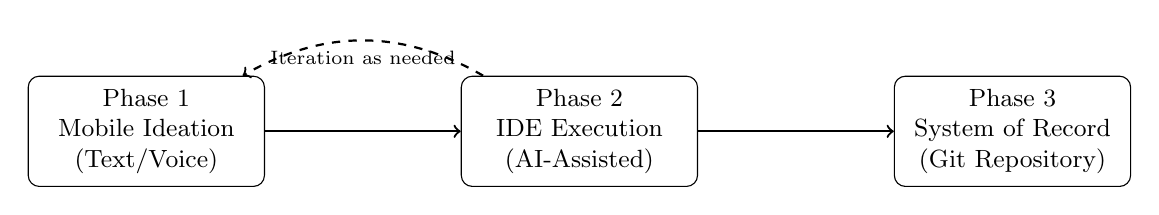
\begin{tikzpicture}[
    box/.style={rectangle, draw, rounded corners, minimum width=3cm, minimum height=1.4cm, align=center, font=\small},
    arrow/.style={->, thick}
]
\node[box] (mobile) at (0,0) {Phase 1\\Mobile Ideation\\(Text/Voice)};
\node[box] (ide) at (5.5,0) {Phase 2\\IDE Execution\\(AI-Assisted)};
\node[box] (git) at (11,0) {Phase 3\\System of Record\\(Git Repository)};

\draw[arrow] (mobile) -- (ide);
\draw[arrow] (ide) -- (git);
\draw[arrow, dashed] (ide) to[bend right=30] node[below, font=\scriptsize] {Iteration as needed} (mobile);
\end{tikzpicture}
\end{center}

\vspace{0.5em}

\begin{columns}
\column{0.33\textwidth}
\textbf{Phase 1: Ideation}
\begin{itemize}
\small
\item Smartphone-based reasoning
\item Text input always available
\item Voice input when possible
\item No controlled data required
\end{itemize}

\column{0.33\textwidth}
\textbf{Phase 2: Execution}
\begin{itemize}
\small
\item Modern IDE environment
\item AI assistance (modular)
\item Within trust boundaries
\item Produces artifacts
\end{itemize}

\column{0.33\textwidth}
\textbf{Phase 3: Record}
\begin{itemize}
\small
\item Git version control
\item Captures history
\item Captures rationale
\item Lifecycle management
\end{itemize}
\end{columns}
\end{frame}

\begin{frame}{Functional Requirements (Solution-Agnostic)}
These requirements define \textit{what} is needed, not \textit{how} to implement it:

\vspace{0.5em}

\begin{table}
\begin{tabular}{@{}llp{8cm}@{}}
\toprule
\textbf{ID} & \textbf{Type} & \textbf{Requirement} \\
\midrule
FR-1 & Mandatory & Mobile ideation capability (smartphone, text/voice input) \\
\addlinespace
FR-2 & Mandatory & IDE-centric execution with integrated, replaceable AI assistance \\
\addlinespace
FR-3 & Mandatory & Git-based system of record capturing artifacts, history, and rationale \\
\addlinespace
FR-4 & Mandatory & Identity and trust boundary alignment (security at identity and device) \\
\addlinespace
FR-5 & Recommended & High-signal communication model (email for notification only) \\
\bottomrule
\end{tabular}
\end{table}

\vspace{0.5em}

\small
Full requirements with verification traceability are in the repository: \texttt{README.md}
\end{frame}

\begin{frame}{Security and Compliance}
SpeakUp maintains existing security posture---no rules are relaxed:

\vspace{0.5em}

\begin{columns}
\column{0.5\textwidth}
\textbf{Trust Boundary Alignment}
\begin{itemize}
\item Security enforced at authenticated identity
\item Security enforced at managed device
\item AI operates in-boundary as assistive tool
\item Classification and handling rules unchanged
\end{itemize}

\column{0.5\textwidth}
\textbf{Information Handling (This Project)}
\begin{itemize}
\item No sensitive PII included
\item No CUI included
\item No proprietary information included
\item No classified information included
\item Verified by inspection (see repository)
\end{itemize}
\end{columns}

\vspace{1em}

\small
Verification evidence: \texttt{verification/Compliance-Statement.md}
\end{frame}

\begin{frame}{Value Proposition}
\begin{block}{The Core Point}
\textbf{With the right environment, one person can do the work of an entire team.}
\end{block}

\vspace{0.5em}

\textbf{Example:} This briefing---IDE, AI agent, LaTeX documents, professional PDFs, version control---all produced by one person. The constraint is not capability. It is environment.

\vspace{0.5em}

\begin{table}
\small
\begin{tabular}{@{}p{3.5cm}p{4.5cm}p{5cm}@{}}
\toprule
\textbf{Capability} & \textbf{Current State} & \textbf{Proposed State} \\
\midrule
Work capture & Fragmented, untracked & Structured, version-controlled \\
\addlinespace
AI assistance & Outside boundary or unavailable & In-boundary, modular \\
\addlinespace
Knowledge preservation & At-risk & Durable artifacts \\
\addlinespace
Automation readiness & Limited & Maximized \\
\addlinespace
Auditability & Manual effort & Built-in traceability \\
\bottomrule
\end{tabular}
\end{table}
\end{frame}

\begin{frame}{Implementation Approach}
This project demonstrates the pattern by being the pattern:

\vspace{1em}

\begin{itemize}
\item \textbf{Concrete enough to execute}
\begin{itemize}
\item Working repository with all artifacts
\item Defined outputs and verification evidence
\item Reproducible workflow documented in \texttt{artifacts/Workflow-Log.md}
\end{itemize}

\vspace{0.5em}

\item \textbf{Abstract enough to remain vendor-neutral}
\begin{itemize}
\item Requirements specify \textit{what}, not \textit{how}
\item Implementation choices documented separately
\item Alternative tools can satisfy same requirements
\end{itemize}

\vspace{0.5em}

\item \textbf{Self-demonstrating}
\begin{itemize}
\item This briefing was created using the proposed workflow
\item Ideation on mobile, execution in IDE, artifacts in Git
\end{itemize}
\end{itemize}

\vspace{0.5em}

\textbf{Example project using this workflow:}\\
\url{https://github.com/brucedombrowski/OpenSourceHouseProject}
\end{frame}

\begin{frame}{Repository Contents}
All project artifacts are available for review:

\vspace{0.5em}

\begin{table}
\begin{tabular}{@{}ll@{}}
\toprule
\textbf{File} & \textbf{Purpose} \\
\midrule
\texttt{README.md} & Authoritative requirements and project specification \\
\addlinespace
\texttt{briefing/SpeakUp-Briefing.pdf} & This document \\
\addlinespace
\texttt{briefing/SpeakUp-Briefing.tex} & Source for this document (version-controlled) \\
\addlinespace
\texttt{verification/Compliance-Statement.md} & Information handling verification evidence \\
\addlinespace
\texttt{verification/Requirements-Traceability.md} & Requirements to evidence mapping \\
\addlinespace
\texttt{artifacts/Workflow-Log.md} & Execution workflow documentation \\
\bottomrule
\end{tabular}
\end{table}

\vspace{0.5em}

\begin{center}
\url{https://github.com/brucedombrowski/SpeakUp}
\end{center}
\end{frame}

\begin{frame}{Verification Summary}
This project produces verification evidence as first-class artifacts:

\vspace{0.5em}

\begin{table}
\begin{tabular}{@{}lll@{}}
\toprule
\textbf{Method} & \textbf{Application} & \textbf{Evidence} \\
\midrule
Inspection & Document review for completeness & Compliance-Statement.md \\
\addlinespace
Analysis & Compliance assessment against requirements & Requirements-Traceability.md \\
\addlinespace
Demonstration & Working repository as proof of concept & This repository \\
\bottomrule
\end{tabular}
\end{table}

\vspace{1em}

\textbf{Key Compliance Findings:}
\begin{itemize}
\item All information handling requirements: \textbf{COMPLIANT}
\item All functional requirements: \textbf{ADDRESSED} or \textbf{DEMONSTRATED}
\item All expected outputs: \textbf{COMPLETE}
\end{itemize}
\end{frame}

\begin{frame}{Recommendation}
\textbf{Adopt the SpeakUp workflow model as a pattern for:}

\vspace{1em}

\begin{itemize}
\item Converting thinking into durable, reviewable artifacts
\item Preserving institutional knowledge as personnel transition
\item Enabling automation and reducing manual audit effort
\item Maintaining security and trust boundaries while using AI assistance
\item Improving signal-to-noise in organizational communication
\end{itemize}

\vspace{1em}

\textbf{This pattern is applicable to:}
\begin{itemize}
\item Engineering work
\item Analytical work
\item Knowledge work generally
\end{itemize}
\end{frame}

\begin{frame}{Next Steps}
\begin{enumerate}
\item \textbf{Review this briefing} and the repository contents
\item \textbf{Identify a pilot application area} where the workflow could be applied
\item \textbf{Establish repository and workflow} for the pilot
\item \textbf{Iterate} between ideation and execution phases
\item \textbf{Measure and refine} based on results
\end{enumerate}

\vspace{1.5em}

\begin{center}
\textit{This briefing was produced using the SpeakUp workflow model it describes.}

\vspace{1em}

\textbf{Repository:} \url{https://github.com/brucedombrowski/SpeakUp}

\vspace{0.5em}

\textbf{Contact:} Bruce Dombrowski (Creator)
\end{center}
\end{frame}

\end{document}
